% \documentclass[]{spie}  %>>> use for US letter paper
\documentclass[a4paper]{spie}  %>>> use this instead for A4 paper
%\documentclass[nocompress]{spie}  %>>> to avoid compression of citations

\renewcommand{\baselinestretch}{1.0} % Change to 1.65 for double spacing
 
\usepackage{amsmath,amsfonts,amssymb}
\usepackage{graphicx}
\usepackage[colorlinks=true, allcolors=blue]{hyperref}
\usepackage{listings}
\usepackage{lstautogobble} % Fix for excessive indentation

\lstset{
    basicstyle=\ttfamily\footnotesize,
    breaklines=true,
    postbreak=\mbox{\textcolor{red}{$\hookrightarrow$}\space},
    frame=single,
    autogobble=true
}


\title{Securing the Software Supply Chain for containers: Practices and Challenges in a Cloud-Native Landscape for a global observatory}

\author[a]{Ugur Yilmaz}
\author[a]{Piers Harding}
\affil[a]{SKA Observatory, United Kingdom}

\authorinfo{Further author information: (Send correspondence to Ugur Yilmaz)\\
Ugur Yilmaz: E-mail: ugur.yilmaz@skao.int\\
Piers Harding: E-mail: piers.harding@skao.int
}

% Option to view page numbers
\pagestyle{empty} % change to \pagestyle{plain} for page numbers   
\setcounter{page}{301} % Set start page numbering at e.g. 301
 
\begin{document} 
\maketitle

\begin{abstract}
In the rapidly evolving landscape of software development the adoption of containerisation has transformed the software supply chain. Containers encapsulate software components, ensuring consistency across multiple development, testing, and production environments. They foster agility and scalability by enabling microservices architecture and DevOps practices. The recent increase in cyberattacks targeting research institutes makes it critical to have a secure supply chain for containers and their orchestration. This paper delves into the integration of containers within the software supply chain, examining best practices and challenges in orchestration, security, and continuous integration and delivery (CI/CD) and distribution. We focus on how containers are secured from build stage, verified and distributed securely and validated in production, while also exploring the implications for dependency management and obsolescence in modern cloud-native infrastructures. Our analysis provides insights into maximising the benefits of containerisation to streamline development pipelines and enhance software supply chain resilience.
\end{abstract}

% Include a list of keywords after the abstract 
\keywords{CI/CD, cybersecurity, kubernetes, cloud, kyverno, notation, policy agent, oci}

\section{INTRODUCTION}
The Square Kilometre Array (SKA) Observatory, one of the most ambitious scientific projects of the 21st century, aims to explore the universe with unprecedented detail and precision. As the observatory's software infrastructure becomes increasingly complex and critical, ensuring the security of its software supply chain has become a paramount concern. The software supply chain encompasses the entire process of developing, packaging, distributing, and maintaining software, from initial development through deployment and updates.

Given the critical role that software plays in the operation and success of the SKA Observatory, protecting the integrity, authenticity, and security of software artefacts is essential. This task is compounded by the reliance on third-party and open-source components and standards, as well as the adoption of containerised applications and cloud-native architectures. The 2021 Executive Order on Improving the Nation's Cybersecurity\cite{ExecutiveOrder14028} and UK Government Cyber Security Strategy\cite{GovernmentCyberSecurity} has further underscored the importance of robust software supply chain security with the increase of cyberattacks \cite{cremerCyberRiskCybersecurity2022}, calling for the use of Software Bill of Materials (SBOMs) and provenance checks. SKA Observatory closely follows the guidance of cloud native landscape alongside with the best practices to ensure it's software supply chain adheres to upmost standards.\cite{CybersecurityFramework2013}

This paper delves into the specific practices and challenges encountered by the SKA Observatory in securing its software supply chain. We will explore each stage of the supply chain, from development and testing to packaging, distribution, and deployment, with a particular emphasis on the unique requirements and constraints of the observatory's environment. Additionally, we will discuss the implementation of critical security measures such as vulnerability scanning, artefact signing, and provenance verification, which are integral to maintaining the security of software in SKA's cloud-native infrastructure.

Through this analysis, we aim to provide a comprehensive overview of the current state of software supply chain security at the SKA Observatory, highlighting both successful practices and ongoing challenges. By sharing these insights, we hope to contribute to the broader discourse on securing scientific software infrastructures and offer practical guidance for other organisations facing similar challenges.

\section{Software Supply Chain Stages at SKA Observatory}

The software supply chain at the SKA Observatory is meticulously structured to ensure the delivery of secure and reliable software artefacts. This process as shown in Figure \ref{fig:stages} spans multiple stages, each with its own set of practices and challenges. Below, we detail each stage of the supply chain and the measures implemented to safeguard the integrity of the software.

SKA Observatory needs to deliver its software into each of its sites, respectively in South Africa and Australia where the deployments for hundreds of dishes and antennas will be driven autonomously in a distributed manner.


% Note: If compiling with LaTeX+dvipdf, please ensure images generated from 
% other software packages have their bounding boxes set correctly.
   \begin{figure} [ht]
   \begin{center}
   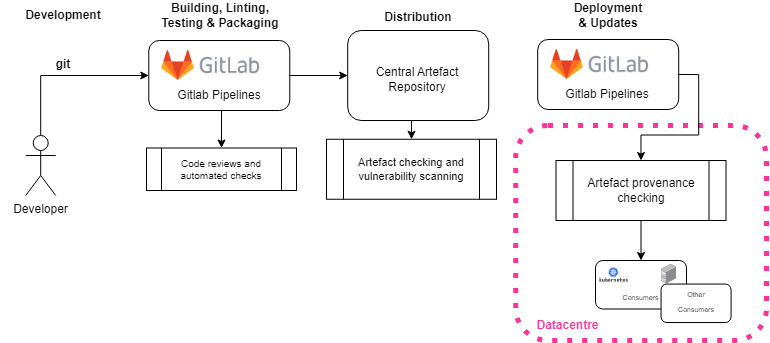
\includegraphics[width=\textwidth,height=\textheight,keepaspectratio]{stages.png}
   \end{center}
   \caption 
%>>>> use \label inside caption to get Fig. number with \ref{}
   { \label{fig:stages}
SKAO Software Supply Chain Stages}
    \end{figure} 

\subsection{Development}

The development stage is the foundation of the software supply chain. At SKA, this stage involves the design and coding of software features, following development guidelines to uphold high-quality standards\cite{SKATelescopeDeveloper}. Developers use secure GitLab\cite{GitLab2024} repositories with enforced access controls and two-factor authentication (2FA) to prevent unauthorised modifications. Code reviews and automated checks, facilitated by tools like Marvin the Paranoid Android\cite{yilmazDrivingBehaviouralChange2023}, ensure adherence to coding standards and identify potential issues early in the development cycle.

\subsection{Building, Linting, and Testing}

Once the code is developed, it undergoes a series of automated processes to ensure quality and functionality. Static checks such as linters are employed to enforce coding standards and detect anti-patterns, while extensive testing—including unit, integration, and system testing—verifies the software's correctness and performance. GitLab runners, operating within the SKA's infrastructure, execute these pipelines, protecting sensitive information and ensuring that builds are conducted in a secure environment.

\subsubsection{Packaging}

Packaging involves bundling the software along with all its dependencies, libraries, configuration and documentation into a distributable format. For the SKA Observatory, this often means creating OCI (Open Container Initiative) images, Python packages, and Helm charts. The packaging process is tightly integrated with the CI/CD pipeline, ensuring that all artefacts are consistently and securely packaged, ready for distribution. During this stage, relevant metadata is added to each package to ensure auditability and traceability related information such as  author, environment, time, Gitlab repository is captured.

\subsection{Distribution}

The distribution stage is critical for making the software artefacts available to various environments. At SKA, distribution is managed through a centralised artefact repository, such as Nexus\cite{SonatypeNexusRepository} or Harbor\cite{Harbor}. These repositories are secured with access controls and authentication mechanisms. Additionally, artefacts are signed to verify their provenance, and vulnerability scanning tools, such as Trivy\cite{TrivyHome}, are used to identify and mitigate potential security risks before the artefacts are deployed.

\subsection{Deployment}

Deployment is the process of installing and configuring the software in target environments. For SKA, this often involves deploying containerised applications to Kubernetes clusters on site and cloud for different purposes. The deployment pipelines are executed on GitLab runners or different deployment mechanisms, ensuring that only verified and approved artefacts are deployed. Deployment configurations and secrets are managed securely to prevent unauthorised access.

   \begin{figure} [ht]
   \begin{center}
   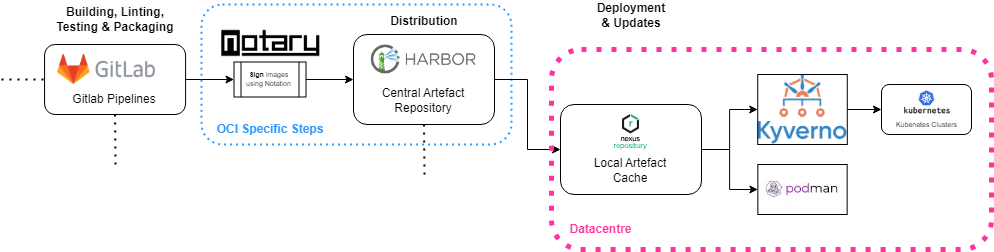
\includegraphics[width=\textwidth,height=\textheight,keepaspectratio]{ssc_oci.png}
   \end{center}
   \caption 
%>>>> use \label inside caption to get Fig. number with \ref{}
   { \label{fig:ssc_oci}
SKAO Software Supply Chain Stages for OCI Images}
    \end{figure} 

Figure \ref{fig:ssc_oci} shows the details of of each steps for OCI images in SKAO infrastructure.

\section{Challenges in Securing the Software Supply Chain}

Despite the robust security measures in place, the SKA Observatory faces several significant challenges in securing its software supply chain. These challenges stem from the complexity of the infrastructure, the distributed nature of the project, the pace of technological change, and the need for compliance with strict standards.

\begin{enumerate}

    \item \textbf{Complexity and Scale:} The SKA Observatory operates a vast and intricate software infrastructure, which spans multiple environments and components across the globe. Managing the security of such a complex system is inherently challenging. Each component and environment must be secured individually, while also ensuring that the entire system operates cohesively. This complexity increases the potential for misconfigurations and vulnerabilities.

    \item \textbf{Third-Party Dependencies:} The reliance on third-party introduces additional risks. While these components can accelerate development and innovation, they also come with potential vulnerabilities and unverified code. Ensuring the security of these dependencies requires constant monitoring, regular updates, and rigorous validation processes to mitigate the risks associated with using external code.

    \item \textbf{Rapid Technological Advancements:} The field of cloud-native technologies and containerisation is evolving rapidly. Keeping pace with these advancements while maintaining a secure software supply chain is a continuous challenge. New tools, frameworks, and best practices emerge frequently, necessitating ongoing learning and adaptation. Additionally, new security threats and vulnerabilities are constantly being discovered, requiring proactive measures to stay ahead of potential risks.

    \item \textbf{Compliance and Standards:} Ensuring compliance with international security standards and regulations adds another layer of complexity. The SKA Observatory must adhere to guidelines from various regulatory bodies, which often involve high level of security requirements. Achieving and maintaining compliance requires comprehensive documentation, regular audits, and continuous improvements to security processes. This can be resource-intensive and requires a dedicated focus on regulatory adherence.

    \item \textbf{Human Factors:} Human error remains a significant challenge in securing the software supply chain. Mistakes in code, misconfigurations, and lapses in following security protocols can introduce vulnerabilities. Mitigating this risk involves implementing comprehensive training programs, promoting a culture of security awareness, and employing automated tools to catch errors that might be overlooked by human eyes.

\end{enumerate}

\section{Security Measures Implemented at SKA Observatory}

To ensure the integrity and security of the software supply chain, the SKA Observatory has implemented a comprehensive set of security measures across all stages of the supply chain. These measures are designed to address potential vulnerabilities and ensure that software artefacts are secure, reliable, and compliant with industry standards.

\subsection{Access Controls and Authentication}

Access control is a fundamental aspect of securing the software supply chain. At SKA, all developers and contributors are required to use two-factor authentication (2FA) when accessing GitLab repositories. Permissions are strictly managed to ensure that only authorised personnel can contribute to specific projects, reducing the risk of unauthorised changes.

\subsection{Code Reviews and Automated Checks}

To maintain high-quality code, the SKA Observatory employs rigorous code review processes. Every merge request undergoes review by peers and automated checks by tools such as Marvin the Paranoid Android. These checks ensure that code adheres to established guidelines, is well-documented, and does not introduce security vulnerabilities.

\subsection{Secure CI/CD Pipelines}

The continuous integration and continuous deployment (CI/CD) pipelines at SKA are executed on secure GitLab runners. These runners operate within the observatory's controlled infrastructure, protecting sensitive information and ensuring that build processes are isolated and secure. The use of dedicated runners instead of shared ones further enhances security by minimising the risk of cross-project contamination.

\subsection{Artefact Signing and Provenance Verification}

To ensure the authenticity and integrity of software artefacts, SKA implements artefact signing. Using tools like Notation\cite{NotaryProject}, artefacts are signed at the time of packaging. This allows downstream consumers to verify the provenance of the artefacts before deployment. Additionally, provenance checks are conducted to ensure that artefacts originate from trusted sources.

\subsection{Vulnerability Scanning}

Before artefacts are distributed, they undergo rigorous vulnerability scanning using tools such as Trivy. This process identifies known vulnerabilities in the artefacts, allowing the SKA team to address these issues before deployment. Regular scanning ensures that artefacts remain secure over time, even as new vulnerabilities are discovered.

\subsection{Secure Deployment Practices}

Deployment at SKA is conducted using mainly GitLab runners, ensuring that only verified and approved artefacts are deployed. Deployment configurations and secrets are managed securely to prevent unauthorised access. Additionally, deployment processes include automated checks to verify the integrity and security of the deployed artefacts.

\subsection{Continuous Monitoring and Security Audits}

Maintaining the security of the software supply chain requires ongoing vigilance. The SKA Observatory employs continuous monitoring and regular security audits to identify and address potential vulnerabilities. Automated systems based on Prometheus\cite{prometheusPrometheusMonitoringSystem}, Grafana\cite{GrafanaOpenObservability} and Elasticsearch\cite{ElasticSearchAI} are used to monitor the security status of deployed software, providing real-time alerts for any anomalies.

\subsection{Compliance with Industry Standards}

Compliance with industry standards and regulations is crucial for ensuring the security of the software supply chain. The SKA Observatory adheres to best practices and standards such as those outlined by the National Institute of Standards and Technology (NIST) and the International Organization for Standardization (ISO). Regular reviews and updates to security policies ensure continued compliance.

\section{Case Studies of Security Challenges}

To illustrate the practical application of the security measures implemented at the SKA Observatory, this section presents several case studies that highlight specific security challenges encountered, the solutions implemented, and the outcomes achieved. These examples provide a deeper understanding of the complexities involved in securing a modern software supply chain in a cloud-native environment.

\subsection{Case Study 1: Addressing Third-Party Vulnerabilities}

\subsubsection{Challenge}

The SKA Observatory is built on the shoulder of giants. It relies heavily on third-party and open-source software components, which can introduce vulnerabilities into the software supply chain. Identifying and mitigating these vulnerabilities is a critical challenge, especially given the dynamic nature of open-source projects and the rapid pace of software updates.

\subsubsection{Solution}

To address this challenge, the SKA Observatory implemented a comprehensive vulnerability scanning process using tools like Trivy\cite{TrivyHome}. All third-party components included in the software builds inside an OCI image are scanned for known vulnerabilities. By default, the observatory does not allow any artefacts with critical vulnerabilities to be deployed. If any critical vulnerabilities are found, they are investigated to identify their impact. Then, they are either accepted or rejected. Moreover, these vulnerability scans are run periodically to catch new vulnerabilities.

To eliminate the most of the vulnerabilities, SKA provides a base OCI image for all the software to be built on. This allows minimum attack surface, enhanced security and hardened OCI images while helping with the software development overhead.

Additionally, the observatory maintains an internal database of approved third-party libraries and continuously monitors for security updates and advisories. Any upstream dependency is first pulled into internal systems where they are vetted. This eliminates man in the middle and package injections attacks from build to production.

\subsubsection{Outcome}

By integrating vulnerability scanning into the CI/CD pipeline, the SKA Observatory was able to significantly reduce the risk of introducing vulnerable components into their software. Regular updates and patches are applied promptly, ensuring that the software remains secure. This proactive approach has led to a notable decrease in security incidents related to third-party vulnerabilities. Developers are also able to see the status of vulnerabilities for their own packages in detail so that they can fix any issues as shown in Figure \ref{fig:harbor}.

   \begin{figure} [ht]
   \begin{center}
   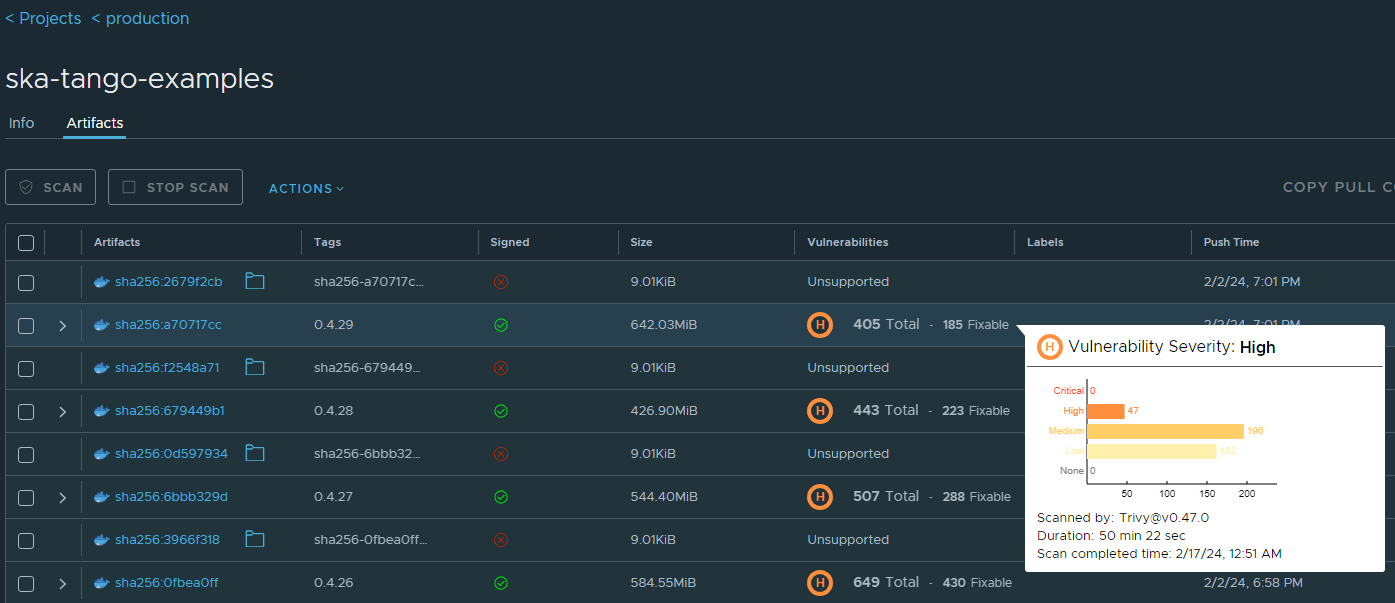
\includegraphics[width=\textwidth,height=\textheight,keepaspectratio]{harbor.png}
   \end{center}
   \caption 
%>>>> use \label inside caption to get Fig. number with \ref{}
   { \label{fig:harbor}
SKAO Harbor OCI Repository}
    \end{figure} 

\subsection{Case Study 2: Ensuring Artefact Integrity with Signing and Verification}

\subsubsection{Challenge}

Ensuring the integrity and authenticity of software artefacts throughout the supply chain is essential to prevent tampering and unauthorised modifications. This is particularly challenging in a distributed environment where artefacts are shared across multiple teams and deployed in various environments.

\subsubsection{Solution}

The SKA Observatory adopted artefact signing using the Notation tool\cite{NotaryProject}, which allows artefacts to be signed during the packaging process. These signatures are then verified at multiple points in the supply chain, including before deployment. This ensures that only verified and trusted artefacts are used in the production environment.

The process of signing and verifying OCI (Open Container Initiative) images involves several key steps:

\paragraph{PKI Setup}
To establish a secure signing infrastructure, we set up a Public Key Infrastructure (PKI), which includes a Certificate Authority (CA), an intermediate CA, and a leaf certificate for signing. The CA and intermediate CA are created using OpenSSL, and the leaf certificate, which will be used for signing, is issued from the intermediate CA.

\begin{lstlisting}
# Generate CA and intermediate CA
mkdir -p root-ca/{certs,crl,newcerts,private} &&  touch root-ca/index.txt && echo 1000 > root-ca/serial
openssl genrsa -aes256 -out ca.key 4096
openssl req -config openssl.cnf -key ca.key -new -x509 -days 36500 -sha256 -extensions v3_ca -out ca.pem
openssl genrsa -aes256 -out oci.interm.key 4096
openssl req -config openssl.cnf -new -sha256 -key oci.interm.key -out oci.interm.csr
openssl ca -config openssl.cnf -extensions v3_intermediate_ca -days 3650 -notext -md sha256 -in oci.interm.csr -out oci.interm.pem
cat oci.interm.pem ca.pem > oci.chain.pem

# Generate leaf certificate
mkdir -p intermediate-ca/{certs,crl,newcerts,private} && touch intermediate-ca/index.txt && echo 1000 > intermediate-ca/serial
openssl genrsa -aes256 -out oci.signer.key 4096
openssl req -config intermediate.openssl.cnf -new -sha256 -key oci.signer.key -out oci.signer.csr
openssl ca -config intermediate.openssl.cnf -extensions v3_signer -days 365 -notext -md sha256 -in oci.signer.csr -out oci.signer.pem
cat oci.signer.pem oci.chain.pem > oci.fullchain.pem
\end{lstlisting}

\paragraph{Signing with Notation}
After setting up the PKI, we use the Notation tool to sign OCI images. This involves adding the CA to the trust store, configuring the signing profile, and then signing the images.

\begin{lstlisting}
# Configure trust store and signing profile
mkdir -p ~/.config/notation/truststore/x509/ca/skao-oci
cp ca.pem ~/.config/notation/truststore/x509/ca/skao-oci/skao-oci.pem
notation certificate list
cp oci.signer.key ~/.config/notation/localkeys/
cp oci.fullchain.pem ~/.config/notation/localkeys/
cat << EOF > ~/.config/notation/signingkeys.json
{
    "default": "skao-oci",
    "keys": [
        {
            "name": "skao-oci",
            "keyPath": "$HOME/.config/notation/localkeys/oci.signer.key",
            "certPath": "$HOME/.config/notation/localkeys/oci.fullchain.pem"
        }
    ]
}
EOF
notation key ls

# Sign the image
notation sign <registry>/<image>:<tag> --key skao-oci
\end{lstlisting}

\paragraph{Validating OCI Image Signatures}
To validate the signed OCI images, a validation policy is configured. This policy ensures that only images signed with trusted keys are accepted.

\begin{lstlisting}
# Configure validation policy
cat << EOF > ./policy.json
{
    "version": "1.0",
    "trustPolicies": [
        {
            "name": "all",
            "registryScopes": [ "*" ],
            "signatureVerification": {
                "level" : "strict"
            },
            "trustStores": [ "ca:skao-oci" ],
            "trustedIdentities": [
                "*"
            ]
        }
    ]
}
EOF
notation policy import ./policy.json

# Verify the image signature
notation verify <registry>/<image>:<tag>
\end{lstlisting}

\paragraph{Policy Agent Integration}
Signed OCI images can be further secured by integrating with a policy agent to enforce signature verification policies within Kubernetes clusters. This ensures that only verified and trusted images are deployed.

By implementing these steps, the SKA Observatory ensures that all OCI images are securely signed and their provenance can be reliably verified, maintaining high standards of security throughout the software supply chain. These steps are done using a short lived certificates that are only valid for the duration of the signing process to ensure the robustness of the signature process itself.

\subsubsection{Outcome}

The implementation of artefact signing and verification has greatly enhanced the integrity and security of the software supply chain. The observatory can now ensure that all deployed artefacts are genuine and have not been tampered with. This measure has increased confidence in the security of the deployed software and reduced the risk of supply chain attacks.

\subsection{Case Study 3: Managing Security in a Cloud-Native Environment}

\subsubsection{Challenge}

Operating in a cloud-native environment introduces unique security challenges, such as securing containerised applications and managing the dynamic nature of cloud resources. Ensuring consistent security policies across multiple cloud environments is a complex task.

\subsubsection{Solution}

To manage these challenges, the SKA Observatory implemented a combination of Kubernetes-native security tools, such as Kyverno\cite{Kyverno} and custom operators. These tools enforce security policies across all Kubernetes clusters, ensuring consistent application of security best practices. Additionally, continuous monitoring and automated compliance checks are used to maintain security across the cloud-native environment.

   \begin{figure} [ht]
   \begin{center}
   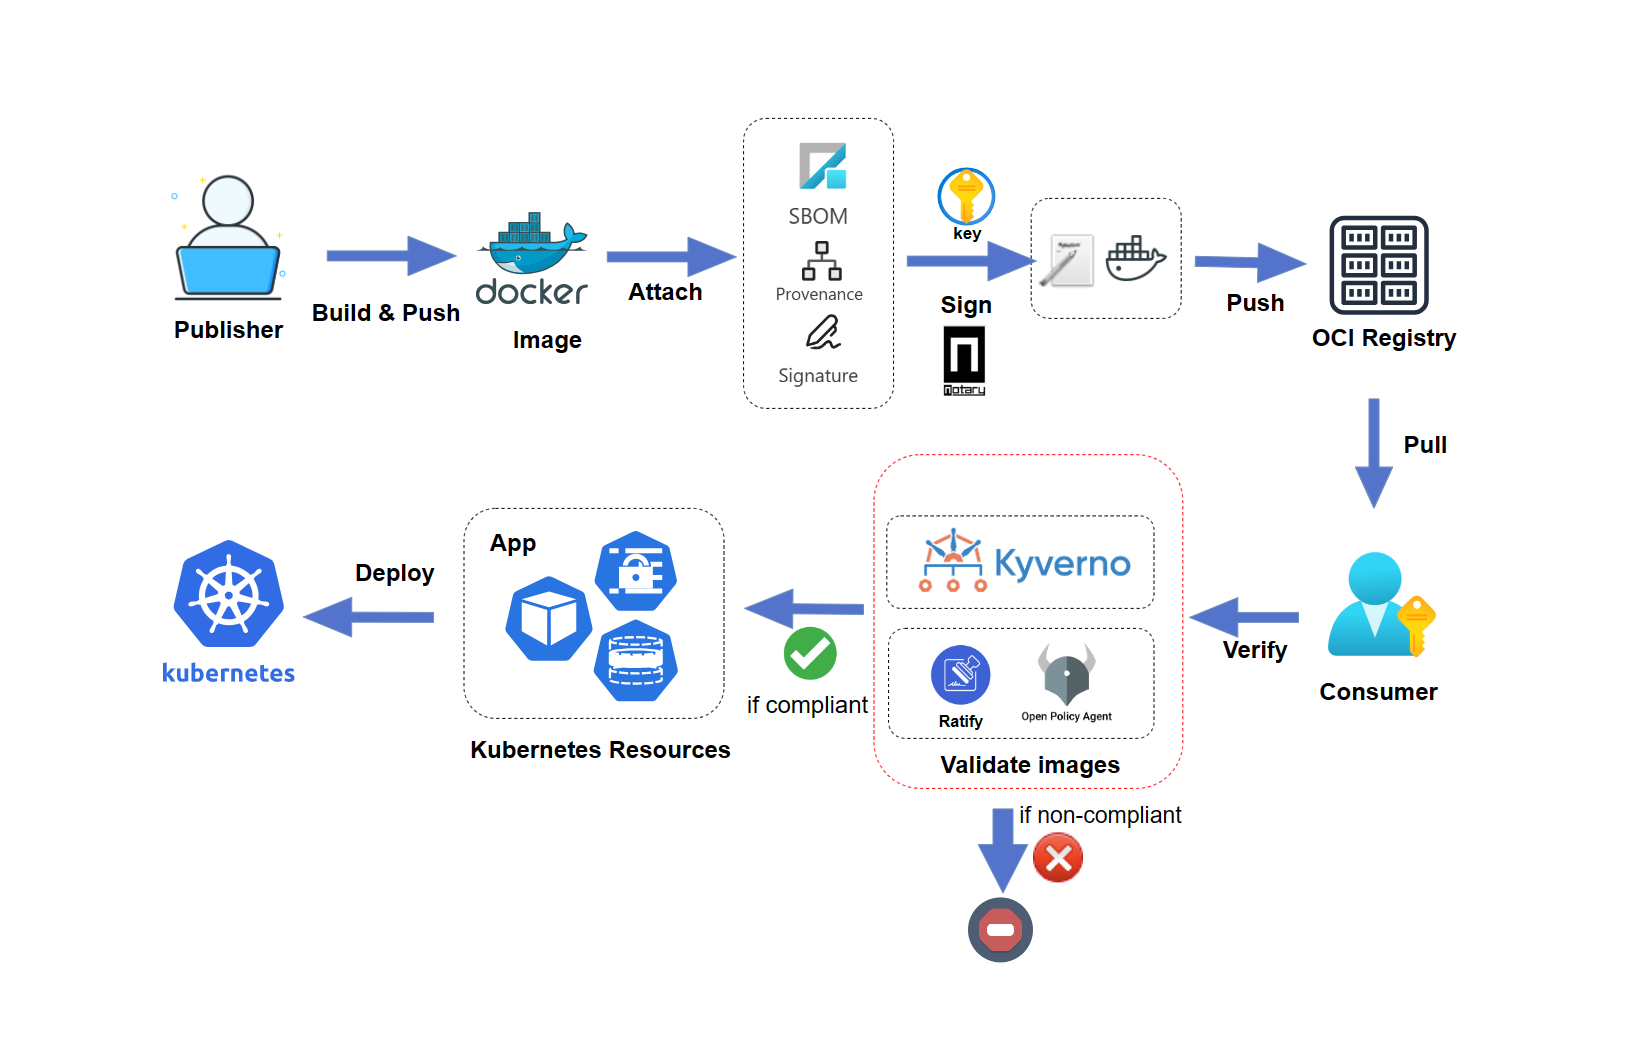
\includegraphics[width=\textwidth,height=\textheight,keepaspectratio]{e2e-workflow.png}
   \end{center}
   \caption 
%>>>> use \label inside caption to get Fig. number with \ref{}
   { \label{fig:chain}
SKAO Harbor OCI Repository}
    \end{figure} 

The process depicted in the Figure \ref{fig:chain} for securing and managing OCI images involves several key steps, which ensure the integrity and security of the software supply chain from creation to deployment. Below is a summarised description of each stage:

\begin{enumerate}
    \item \textbf{Publisher}:
    \begin{itemize}
        \item \textbf{Build \& Push}: The publisher builds an OCI image and pushes it to the registry.
    \end{itemize}
    
    \item \textbf{Attach}:
    \begin{itemize}
        \item The built image is attached with a Software Bill of Materials (SBOM) and provenance information.
    \end{itemize}
    
    \item \textbf{Sign}:
    \begin{itemize}
        \item The image is signed using a key, with Notation.
    \end{itemize}
    
    \item \textbf{Push}:
    \begin{itemize}
        \item The signed image is pushed to the Harbor registry.
    \end{itemize}
    
    \item \textbf{Pull}:
    \begin{itemize}
        \item Consumers pull the image from the OCI registry.
    \end{itemize}
    
    \item \textbf{Verify}:
    \begin{itemize}
        \item The consumer verifies the signature of the pulled image to ensure its integrity and authenticity.
    \end{itemize}
    
    \item \textbf{Validate Images}:
    \begin{itemize}
        \item The image undergoes validation using Kyverno.
        \item If the image is compliant, it is approved for deployment.
    \end{itemize}
    
    \item \textbf{Kubernetes}:
    \begin{itemize}
        \item \textbf{Deploy}: The compliant image is deployed to Kubernetes clusters.
        \item The image becomes part of the Kubernetes resources and applications.
    \end{itemize}
    
    \item \textbf{Non-compliance}:
    \begin{itemize}
        \item If the image is non-compliant during validation, it is blocked from being deployed.
    \end{itemize}
\end{enumerate}

This process ensures that only verified and compliant images are deployed to Kubernetes clusters, maintaining the security and integrity of the software supply chain.

\subsubsection{Outcome}

The adoption of Kubernetes-native security tools has enabled the SKA Observatory to maintain a robust security posture in a cloud-native environment. Consistent policy enforcement and automated compliance checks have improved the overall security and reduced the administrative burden of managing security across multiple environments. This approach has resulted in a more secure and resilient software infrastructure.

\section{Lessons Learned}

Introducing an image signing and verification process adds additional steps to the CI/CD pipeline, which can increase operational overheads and complexity. This includes setting up and maintaining the PKI infrastructure, integrating signing and verification tools, and ensuring all software developers are aware of the new processes and can follow.

SKAO already had a Nexus based system in place where images were scanned but not signed. As part of this effort, Harbor was deployed and existing images had to be migrated with very little downtime. 


All the existing images were signed manually and pushed into the Harbor to have them continue to be used. The Harbor URL and Nexus URL was kept in sync so that image name and tags do not need to be updated.

Setting up a robust PKI infrastructure involves generating and managing multiple certificates, configuring signing tools, and ensuring they are integrated with existing CI/CD workflows. This required significant upfront effort and expertise to get it right with all the edge cases of using microservices based architecture across many time zones.


\section{Future Directions and Conclusion}

The SKA Observatory continues to evolve its approach to securing the software supply chain, with several initiatives planned for the future. These include further automation of security processes, integration of SBOMs, and extending the secure software supply chain to other kinds of artefacts such as python packages and Helm charts.

In conclusion, securing the software supply chain in a cloud-native environment is a multifaceted challenge that requires a comprehensive and proactive approach. By implementing security measures at every stage of the supply chain, the SKA Observatory has successfully mitigated many of the risks associated with modern software development and deployment. The case studies presented in this paper demonstrate the effectiveness of these measures and provide valuable insights for other organisations facing similar challenges.

% References
\bibliography{report} % bibliography data in report.bib
\bibliographystyle{spiebib} % makes bibtex use spiebib.bst

\end{document} 
